Für die folgenden Experimente liegen keine Messwerte vor. Sie eignen sich aber, dank der Tatsache, dass bestimmte Verhaltensmuster erwartet werden, zum Überprüfen, ob der CoDy Algorithmus richtig implementiert wurde.

Für jedes Experiment wird zuerst geklärt, was mit diesem gezeigt werden soll. Darauf folgend wird der Aufbau des Experiments beschrieben und die zu erwartenden Beobachtungen vorgestellt. Abschließend werden, für alle Experimente zusammenfassend, die eigenen Beobachtungen vorgestellt.

Für alle Experimente dieses Kapitel gilt die Erwartungshaltung, dass alle 30 Durchläufe erfolgreich absolviert werden.

%
\subsection{Kurze Engstelle}
\label{chap:engstelle}
Mit diesem Experiment wird gezeigt, dass Agenten Ausweichbewegungen durchführen und Wartephasen einlegen, um andere Agenten passieren zu lassen.

\textbf{Aufbau des Experiments}
\begin{figure}[H]
    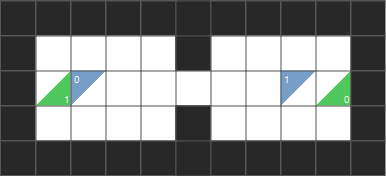
\includegraphics[height=40mm]{images/one_slit.png}
    \centering
    \caption{Aufbau für das Durchfahren zweier Agenten durch eine kurze Engstelle}
    \label{fig:engstelle}
\end{figure}
Die Karte misst neun mal drei Felder. In der Mitte der Karte ist eine eins mal eins Feld breite Engstelle. Auf beiden Seiten dieser Engstelle stehen sich Agenten gegenüber, die die Engstelle durchfahren müssen, um ihre Zielposition zu erreichen.

\textbf{Erwartete Beobachtungen}\newline
Der Agent, der zuerst einen Weg plant, fährt direkt auf seine Zielposition. Der andere Agent fährt eine Ausweichposition in der unmittelbaren Nähe der Engstelle an. Nachdem der erste Agent die Engstelle passiert hat, wird sich der zweite Agent auf direkten Weg zu seinem Ziel machen.
%
\subsection{Umweg}
\label{chap:umweg}
Hier wird gezeigt wie ein Agent einen anderen verdrängt, aber auch das Agenten Umwege in Kauf nehmen.

\textbf{Aufbau des Experiments}
\begin{figure}[H]
    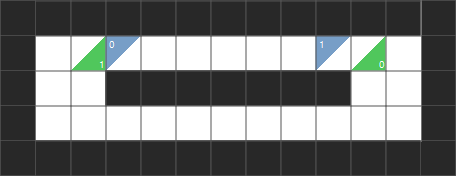
\includegraphics[height=40mm]{images/detour.png}
    \centering
    \caption{Aufbau für ein Szenario, in dem ein Agent einen Umweg in Kauf nimmt}
    \label{fig:umweg}
\end{figure}
Die Karte in Abbildung \ref{fig:umweg} misst elf mal drei Felder und wird mittig, horizontal durch einen Streifen aus sieben Feldern getrennt. Die Start- und Zielpositionen der Agenten sind so angeordnet, dass die nördliche Engstelle den kürzeren Weg darstellt und die südliche Engstelle den Umweg.

\textbf{Erwartete Beobachtungen}\newline
Für kleine Umgebungskarten, also solche bei denen sich die Umgebungskarten der beiden Agenten erst nach dem Annähern überlappen, werden sich beide Agenten in der nördlichen Engstelle annähern. Wenn sich die Umgebungskarten dann überlappen, wird einer der Agenten den Zuschlag erhalten und den anderen Agenten verdrängen. Dieser wird dann über die südliche Engstelle, also über den Umweg, sein Ziel anfahren.

Für größere Umgebungskarten wird der Agent, der zuerst seinen Weg plant, direkt und der andere über den Umweg sein Ziel anfahren.
%
\subsection{Tunnel}
\label{chap:tunnel}
Dieses Experiment testet, wie anfällig die Agenten für Verklemmungen sind.

\textbf{Aufbau des Experiments}
\begin{figure}[H]
    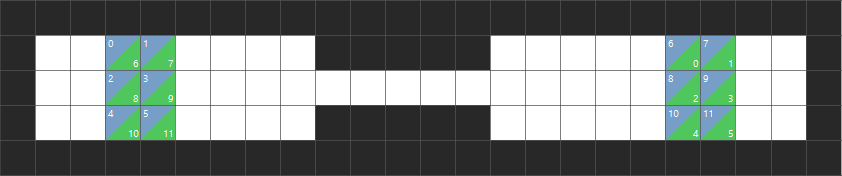
\includegraphics[width=\textwidth]{images/tunnel_2_groups.png}
    \centering
    \caption{Ausgangssituation für das Durchqueren eines Tunnels von zwei Gruppen, bestehend aus jeweils sechs Agenten}
    \label{fig:tunnel}
\end{figure}
In diesem Experiment durchqueren zwei Gruppen aus jeweils sechs Agenten eine Engstelle, die fünf Felder lang und ein Feld breit ist. Jeder Agent muss die Engstelle passieren um sein Ziel zu erreichen.

\textbf{Erwartete Beobachtungen}\newline
Im ersten Schritt nähern sich beide Gruppen der Engstelle. Während eine Gruppe anfängt die Engstelle zu durchqueren, fahren die Agenten der anderen Gruppe Ausweichpositionen an und verlängern damit die Engstelle. Im Laufe des Experiments wechseln die Gruppen ihre Rollen häufiger.
%
\subsection{Tunnel mit kleiner Ausweichbucht}
\label{chap:ausweichbucht}
Dieses Experiment dient zur Veranschaulichung der dynamischen Prioritäten. Diese Situation kann, dezentral, nämlich nicht durch feste Prioritäten gelöst werden.

\textbf{Aufbau des Experiments}
\begin{figure}[H]
    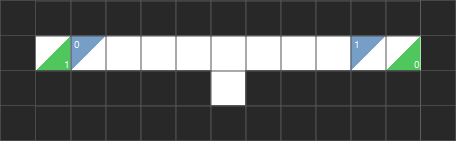
\includegraphics[height=32mm]{images/tunnel_turnout.png}
    \centering
    \caption{Aufbau für die Vorbeifahrt zweier Agenten in einem Tunnel mit einer kleinen Ausweichbucht}
    \label{fig:ausweichbucht}
\end{figure}
Zwei sich gegenüberstehende Agenten versuchen, in einer elf Felder langen und ein Feld schmalen Engstelle aneinander vorbei auf ihre Zielpositionen zu fahren. Der Tunnel hat in der Mitte ein zusätzliches freies Feld, das von den Agenten genutzt werden muss, um aneinander vorbei zu fahren.

\textbf{Erwartete Beobachtungen}\newline
Zuerst werden die beiden Agenten aufeinander zu fahren. Dann wird einer der beiden Agenten zurückgedrängt werden. Wenn der zurückgedrängte Agent sich nicht weiter zurückdrängen lässt, wird dieser seine Priorität erhöhen und den zu erst drängenden Agenten in die Ausweichbucht drängen, was dann beiden Agenten ermöglicht aneinander vorbei zu ihren Zielpositionen zu fahren. Es kann auch passieren, dass ein Agent die Ausweichbucht direkt anfährt und es zu keiner Verdrängung kommt.
%
\subsection{Durchfahren einer stehenden Menge}
\label{chap:menge}
In diesem Experiment wird gezeigt, dass obwohl ein Agent sein Ziel schon erreicht hat, immer noch aktiv an der passiven Kooperation teilnimmt.

\textbf{Aufbau des Experiments}
\begin{figure}[H]
    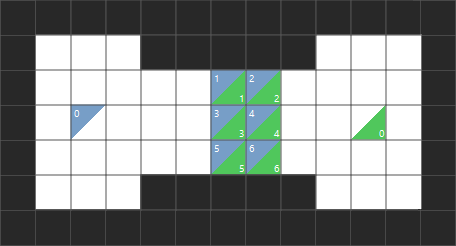
\includegraphics[height=56mm]{images/crowd_drive-through.png}
    \centering
    \caption{Aufbau für das Durchfahren eines Agenten durch ein Menge stehender Agenten}
    \label{fig:menge}
\end{figure}
Die Abbildung \ref{fig:menge} zeigt die Karte für dieses Experiment. Diese hat Dimensionen von elf mal fünf Felder. In der Mitte ist eine fünf Felder lange und drei Felder breite Engstelle. In dieser Engstelle stehen in zwei Reihen hintereinander sechs Agenten. Die Startpositionen dieser Agenten sind gleichzeitig ihre Zielpositionen. Ein weiterer Agent hat seine Startposition auf der linken Seite der Engstelle und seine Zielposition auf der Rechten. Er muss also durch die stehende Menge, um sein Ziel zu erreichen.

\textbf{Erwartete Beobachtungen}\newline
Die Agenten "'3"' und "'4"' werden von Agent "'0"' verdrängt, fahren also von ihren Zielpositionen weg, um Platz für Agent "'0"' zu machen. Es ist auch möglich, dass dabei andere Agenten von ihren Zielpositionen verdrängt werden. Nachdem Agent "'0"' die Menge durchquert hat, fahren alle Agenten wieder zurück zu ihren Zielpositionen.
%
\subsection{Kreuzung}
\label{chap:kreuzung}
Dieses Szenario dient der Beobachtung der Flexibilität der Agenten. Außerdem soll der Unterschied zu einem zentralen Ansatz deutlich gemacht werden und die Skalierbarkeit des Ansatzes gezeigt werden.

\textbf{Aufbau des Experiments}
\begin{figure}[H]
    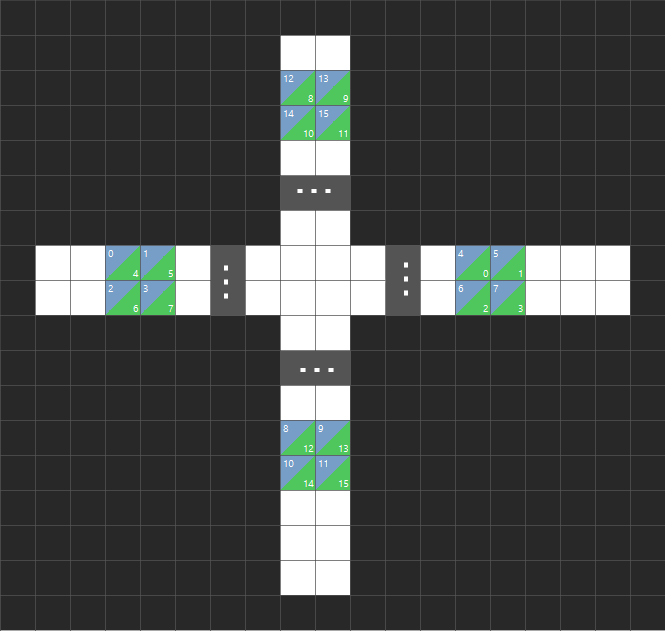
\includegraphics[width=\textwidth]{images/junction.png}
    \centering
    \caption{Aufbau für das Passieren einer Kreuzung von vier Gruppen, bestehend aus jeweils vier Agenten}
    \label{fig:kreuzung}
\end{figure}
In diesem Experiment versuchen vier Gruppen von jeweils vier Agenten eine Kreuzung zu durchqueren. Ziel jeder Gruppe ist es, die gegenüberliegende Seite in gleicher Formation zu erreichen. Der Kreuzungsbereich besteht aus acht freien Feldern, bietet also nicht genügend Platz für alle Agenten. Normale Verkehrsregeln, zum Beispiel das Rechtsfahrgebot, Vorfahrtsregeln oder das Bilden von Fahrspuren, sind keine Lösungen, die ein konfliktfreies aneinander Vorbeifahren der Agenten ermöglichen. Die vier Fahrbahnen der Kreuzung sind jeweils zwei Felder breit und 14 Felder lang.

\textbf{Erwartete Beobachtungen}\newline
Wegen der dynamischem Prioritäten ist eine Vielzahl an Lösungen zu beobachten. Der Berechnungsaufwand pro Agent steigt, trotz der gestiegenen Teilnehmerzahl, nicht.
Ein möglicher zentraler Ansatz würde vermutlich zwei Gruppen blockieren und die übrigen gegenüberliegenden Gruppen durch die Kreuzung passieren lassen, um erst danach den blockierten Gruppen die Durchfahrt zu gewähren. Dies ist vergleichbar mit einer Ampel an einer Kreuzung im Straßenverkehr.


%
\subsection{Beobachtungen}
\label{chap:beobachtungen}
Alle zu erwartenden Beobachtungen konnten, so wie in \cite{book:regele} beschrieben, in den eigens ausgeführten Experimenten beobachtet werden.
